\documentclass[a4paper, 12pt]{extreport}
\usepackage[utf8]{inputenc}
\usepackage[english,russian]{babel}
\usepackage{amssymb,amsfonts,amsmath,mathtext,cite,enumerate,float}
\usepackage{pgfplots}
\usepackage{graphicx}
\usepackage[inkscapeformat=png]{svg}
\usepackage{tocloft}
\usepackage{listings}
\usepackage{caption}
\usepackage{tempora}
\usepackage{titlesec}
\usepackage{setspace}
\usepackage{geometry}
\usepackage{indentfirst}
\usepackage{pdfpages}
\usepackage{enumerate,letltxmacro}
\usepackage{threeparttable}
\usepackage{hyperref}
\usepackage{flafter}
\usepackage{enumitem}
\usepackage{multirow}
\usepackage{mathtools}
\usepackage{longtable}
\usepackage[figure,table]{totalcount}
\usepackage{lastpage}

\lstdefinestyle{code}{
	basicstyle=\footnotesize\ttfamily,
	frame=single,
	tabsize=4,	
	breaklines=true
}

\setlist{nosep}
\hypersetup{pdfborder=0 0 0}

\newcommand{\ssr}[1]{\begin{center}
		\LARGE\bfseries{#1}
	\end{center} \addcontentsline{toc}{chapter}{#1}  }

\makeatletter
\renewcommand\LARGE{\@setfontsize\LARGE{22pt}{20}}
\renewcommand\Large{\@setfontsize\Large{20pt}{20}}
\renewcommand\large{\@setfontsize\large{16pt}{20}}
\makeatother

\RequirePackage{titlesec}
\titleformat{\chapter}[block]{\hspace{\parindent}\large\bfseries}{\thechapter}{0.5em}{\large\bfseries\raggedright}
\titleformat{name=\chapter,numberless}[block]{\hspace{\parindent}}{}{0pt}{\large\bfseries\centering}
\titleformat{\section}[block]{\hspace{\parindent}\large\bfseries}{\thesection}{0.5em}{\large\bfseries\raggedright}
\titleformat{\subsection}[block]{\hspace{\parindent}\large\bfseries}{\thesubsection}{0.5em}{\large\bfseries\raggedright}
\titleformat{\subsubsection}[block]{\hspace{\parindent}\large\bfseries}{\thesubsection}{0.5em}{\large\bfseries\raggedright}
\titlespacing{\chapter}{12.5mm}{-22pt}{10pt}
\titlespacing{\section}{12.5mm}{10pt}{10pt}
\titlespacing{\subsection}{12.5mm}{10pt}{10pt}
\titlespacing{\subsubsection}{12.5mm}{10pt}{10pt}

\makeatletter
\renewcommand{\@biblabel}[1]{#1.}
\makeatother

\geometry{left=30mm}
\geometry{right=10mm}
\geometry{top=20mm}
\geometry{bottom=20mm}

\onehalfspacing

\renewcommand{\theenumi}{\arabic{enumi}}
\renewcommand{\labelenumi}{\arabic{enumi}\text{)}}
\renewcommand{\theenumii}{.\arabic{enumii}}
\renewcommand{\labelenumii}{\asbuk{enumii}\text{)}}
\renewcommand{\theenumiii}{.\arabic{enumiii}}
\renewcommand{\labelenumiii}{\arabic{enumi}.\arabic{enumii}.\arabic{enumiii}.}

\renewcommand{\cftchapleader}{\cftdotfill{\cftdotsep}}

\addto\captionsrussian{\renewcommand{\figurename}{Рисунок}}
\DeclareCaptionLabelSeparator{dash}{~---~}
\captionsetup{labelsep=dash}

\captionsetup[figure]{justification=centering,labelsep=dash}
\captionsetup[table]{labelsep=dash,justification=raggedright,singlelinecheck=off}
\captionsetup[lstlisting]{labelsep=dash,justification=raggedright,singlelinecheck=off}

\newcommand{\floor}[1]{\lfloor #1 \rfloor}

\pgfplotsset{width=0.85\linewidth, height=0.5\columnwidth}

\linespread{1.3}

\parindent=1.25cm

\def\labelitemi{---}
\setlist[itemize]{leftmargin=1.25cm, itemindent=0.65cm}
\setlist[enumerate]{leftmargin=1.25cm, itemindent=0.55cm}

\newcommand{\specialcell}[2][c]{%
	\begin{tabular}[#1]{@{}c@{}}#2\end{tabular}}
\frenchspacing


\begin{document}
\begin{titlepage}
	\newgeometry{pdftex, left=2cm, right=2cm, top=2.5cm, bottom=2.5cm}
	\fontsize{12pt}{12pt}\selectfont
	\noindent\begin{tabular}{|c|c|}	\hline
	\noindent\begin{minipage}{0.15\textwidth}
		
\includegraphics[width=\linewidth]{tools/logo.png}
	\end{minipage} &
	\noindent\begin{minipage}{0.85\textwidth}\centering
		\textbf{\newline Министерство науки и высшего образования Российской Федерации}\\
		\textbf{Федеральное государственное бюджетное образовательное учреждение высшего образования}\\
		\textbf{«Московский государственный технический университет имени Н.Э.~Баумана}\\
		\textbf{(национальный исследовательский университет)»}\\
		\textbf{(МГТУ им. Н.Э.~Баумана)}
	\end{minipage} \\
	\hline	\end{tabular}\newline\newline\newline
	\noindent ФАКУЛЬТЕТ \underline{«Информатика и системы управления»} \newline\newline
	\noindent КАФЕДРА \underline{«Программное обеспечение ЭВМ и информационные технологии»}\newline\newline\newline\newline\newline\newline

	\noindent\begin{minipage}{1.0\textwidth}\centering
		\Large\textbf{       Лабораторная работа №5}
		\end{minipage}
		
	\noindent\begin{minipage}{1.0\textwidth}\centering
		\textbf{\newline}	
		\end{minipage}

	\noindent\begin{minipage}{1.0\textwidth}\centering
		\Large\textbf{по дисциплине «Анализ алгоритмов»}	
		\end{minipage}
		
	\noindent\begin{minipage}{1.0\textwidth}\centering
		\Large\textbf{\newline\newline\newline\newline}	
		\end{minipage}
		
	\noindent\textbf{Тема} \underline{Организация параллельных вычислений по конвейерному принципу}\newline\newline
	\textbf{Студент} \underline{Тузов Даниил Александрович}\newline\newline
	\textbf{Группа} \underline{ИУ7-52Б}\newline\newline
	\textbf{Преподаватель} \underline{Строганов Дмитрий Владимирович}
	
	\begin{center}
		\vfill
		Москва, \the\year~г.
	\end{center}
	\restoregeometry
	\clearpage
\end{titlepage}

\setlength{\cftbeforetoctitleskip}{-4mm}
\renewcommand{\contentsname}{\makebox[\textwidth][c]{СОДЕРЖАНИЕ}}
\tableofcontents
\setcounter{page}{2}

\clearpage\ssr{ВВЕДЕНИЕ}

В 5 лабораторной работе рассматривается тема обработки задач по конвейерному принципу.

Параллелизм описывает последовательности действий, которые происходят одновременно~\cite{parallel}. Нередко в 
современных системах используется распараллеливание вычислений, которое может привести к росту временной 
эффективности программы.

Целью работы является разработка ПО, выполняющего обработку файлов с html-кодом рецептов с сайта~\cite{reciept} в
конвейерном режиме. Для достижения поставленной цели необходимо решить следующие задачи:
\begin{itemize}
	\item[---] рассмотреть структуру сайта;
	\item[---] разработать ПО, обрабатывающее файлы с html-кодом в конвейерном режиме: чтение, парсинг и запись в json
	файл;
	\item[---] исследовать лог времен создания, поступления в очередь, обработки и уничтожения каждой задачи;
	\item[---] сформировать базу данных по полученным json-файлам;
	\item[---] обосновать полученные результаты.
\end{itemize}

\chapter{Входные и выходные данные}

Входными данными в программе является директория с файлами, содержащими HTML-код страницы с рецептом. Выходными
данными является директория с файлами в формате json, в которых хранится информация о:
\begin{itemize}
	\item[---] названии;
	\item[---] авторе;
	\item[---] ингредиентах;
	\item[---] шагах выполнения;
\end{itemize}

\chapter{Преобразование входных данных в выходные}

Программа написана на языке C++ с использованием объектно-ориентированного программирования. Класс-конвейер 
моделирует работу конвейера. Для этого внутри функции $execute$ создается 3 отдельных потока \cite{threads}, отвечающих за 
обработку на каждой стадии и поток-диспетчер, отвечающий за создание задач. Пример кода представлен в листинге 
\ref{lst:class}:

\begin{lstlisting}[style=code, label=lst:class,caption=Класс-конвейер]
class Conveyer {
public:
	Conveyer(int col_files);
	void execute();
	void generate();
	void first_process();
	void second_process();
	void third_process();
private:
	std::queue<std::shared_ptr<ConveyerTask>> _first_queue;
	std::queue<std::shared_ptr<ConveyerTask>> _second_queue;
	std::queue<std::shared_ptr<ConveyerTask>> _third_queue;
	std::thread _threads[4];
	std::vector<std::shared_ptr<ConveyerTask>> _pool_tasks;
	std::vector<std::string> _urls;
	std::shared_ptr<Logger> _logger;
	int _col_files;
};
\end{lstlisting}

После формирования директории с файлами в формате json запускается скрипт на языке Python~\cite{python3} для 
формирования базы данных PostgreSQL~\cite{pgsql}. Код приведен в листинге \ref{lst:database}:

\begin{lstlisting}[style=code, label=lst:database,caption=Скрипт-создающих таблицу в базе данных]
import psycopg2
from os import listdir
from os.path import isfile, join

class Lab:
    def __init__(self):
        self.__conn = psycopg2.connect(dbname="postgres",
                                      user="postgres",
                                      password="postgres123",
                                      host="localhost")
        self.__cursor = self.__conn.cursor()

    def __del__(self):
        self.__cursor.close()
        self.__conn.close()

    def create_db_request(self):
        sql_cr_schema = """create schema if not exists aalab;"""
        self.__cursor.execute(sql_cr_schema)
        sql_cr_table = """
            create table if not exists aalab.parse (
                id integer,
                issue_id integer,
                url text,
                title text,
                author text,
                ingredients json,
                steps json
            );
            alter table aalab.parse add constraint id_pk primary key(id);"""
        self.__cursor.execute(sql_cr_table)
        files = [join("data_json", f) for f in listdir("data_json") if isfile(join("data_json", f))]
        for i in files:
            sql_add_file = "create temp table tmp ( tmp json );\n" + \
                f"copy tmp from 'D:\Study\AA_labs\lab_5\\{i}';\n" + \
                "insert into aalab.parse\n" + \
                "select (json_populate_record(null::aalab.parse, json_array_elements(tmp))).* from tmp;\n" + \
                "drop table tmp;"
            self.__cursor.execute(sql_add_file)
        self.__conn.commit()

db = Lab()
db.create_db_request()
\end{lstlisting}

\chapter{Тестирование}

При тестировании программы на вход подавалось число задач, которые необходимо обработать, и директория с файлами с 
html-кодом. В результате работы формировалась директория с файлами в формате json . На следующем этапе 
выполнялось сравнение файла с html кодом с json-файлом полученном в результате работы, проверялось успешность парсинга.

Тестирования выполнялось для разного количества задач.

Все тесты успешно пройдены.

\chapter{Примеры работы программы}

На рисунке \ref{pic:in} представлен исходный файл:
\begin{figure}[h]
	\centering
	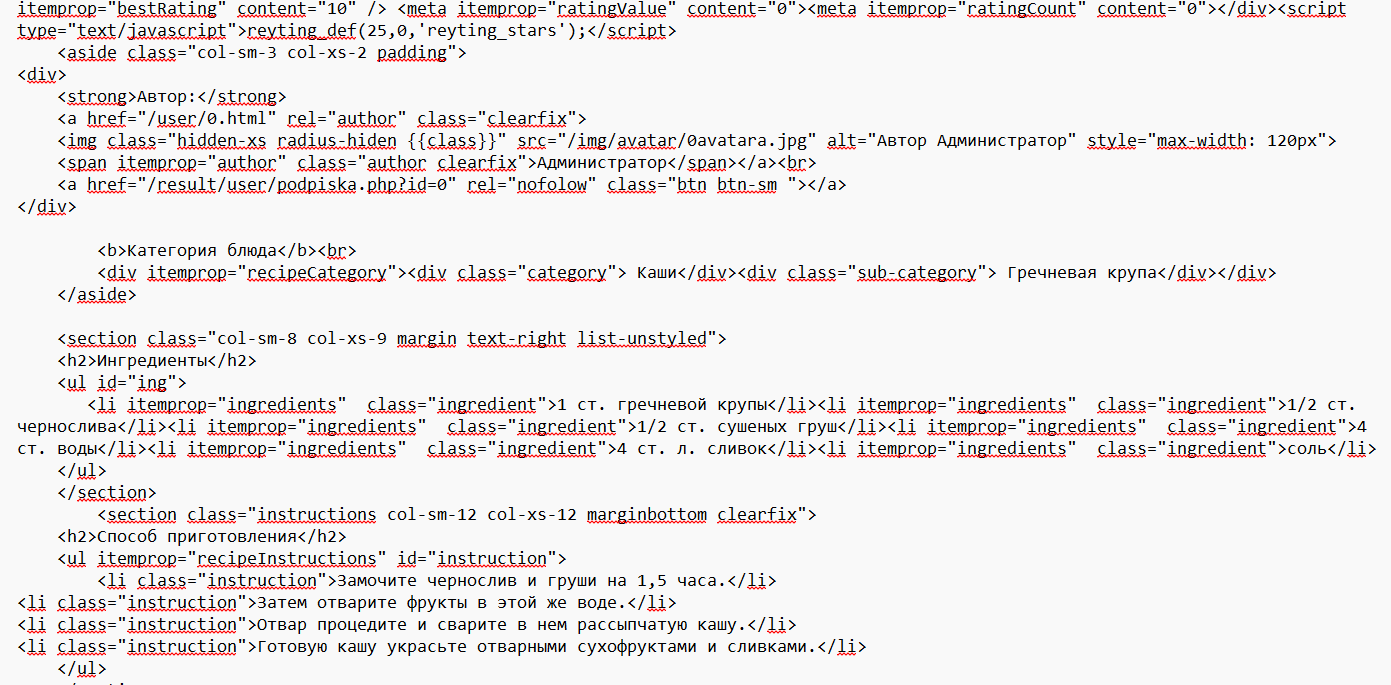
\includegraphics[scale=0.5]{tools/in.png}
	\caption{Файл, содержащий html-код страницы рецепта}
	\label{pic:in}
\end{figure}

На рисунке \ref{pic:out} представлен json-файл:
\begin{figure}[h]
	\centering
	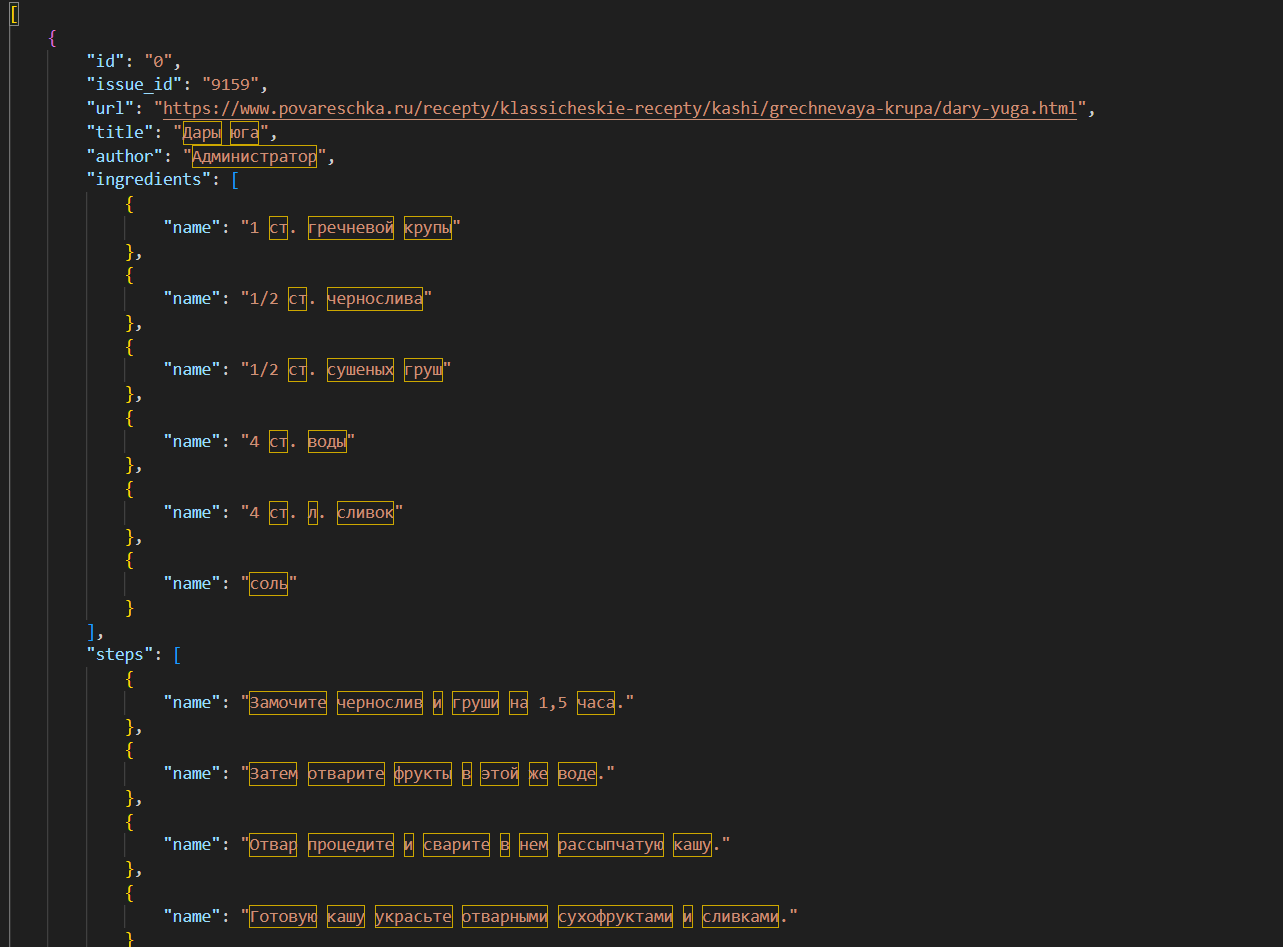
\includegraphics[scale=0.5]{tools/out.png}
	\caption{Файл, содержащий json-код рецепта}
	\label{pic:out}
\end{figure}

На рисунке \ref{pic:db} представлена таблица в базе данных:
\begin{figure}[h]
	\centering
	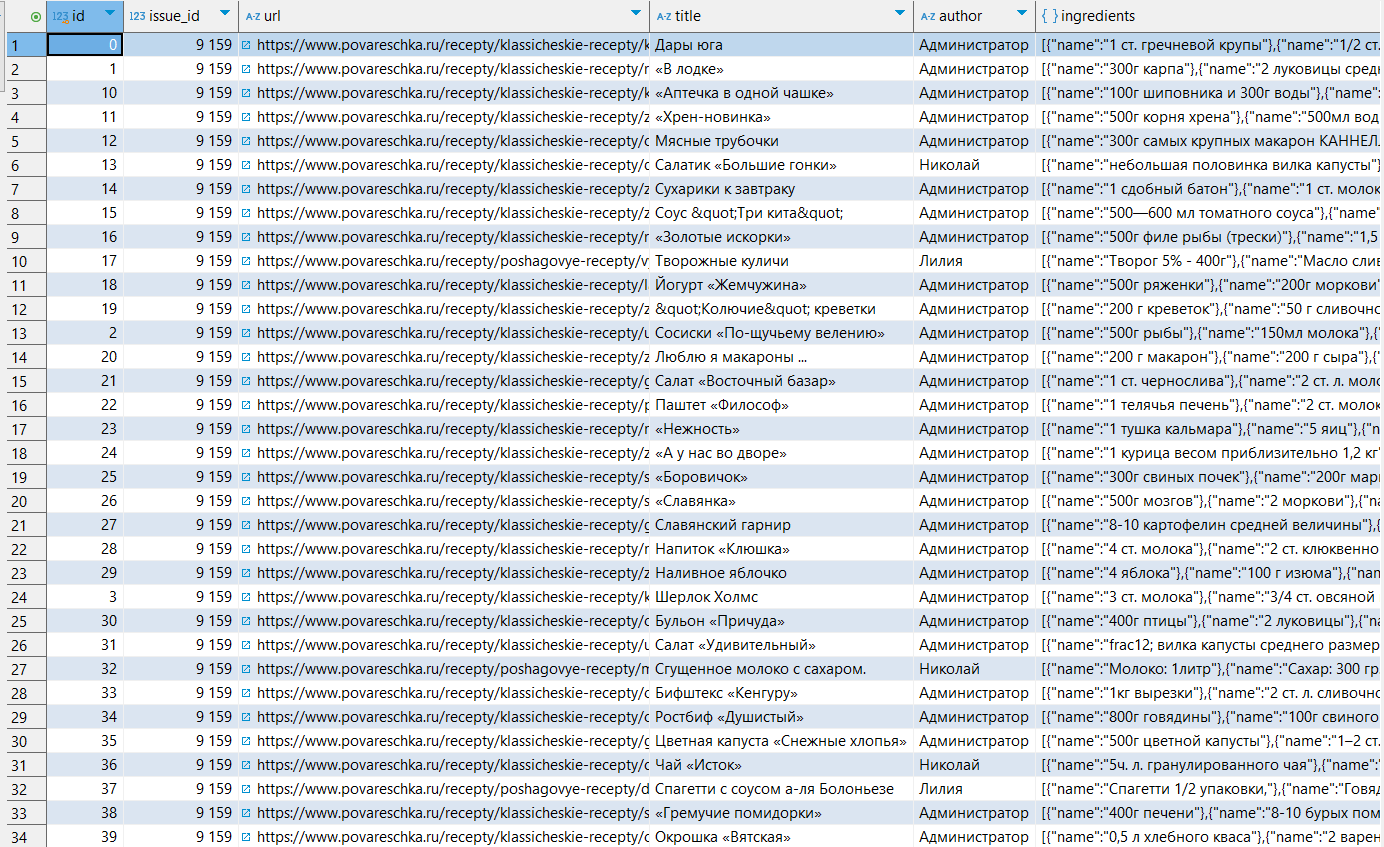
\includegraphics[scale=0.5]{tools/db.png}
	\caption{Сформированная БД}
	\label{pic:db}
\end{figure}

\chapter{Описание исследования}

Все замеры проводились на ЭВМ, характеристики которой приведены ниже:
\begin{itemize}
	\item[---] процессор -- 12th Gen Intel(R) Core(TM) i5-12450H   2.00 ГГц;
	\item[---] оперативная память -- 16,0 ГБ;
	\item[---] тип системы -- 64-разрядная операционная система, процессор x64;
	\item[---] операционная система -- Windows 11;
	\item[---] версия ОС -- 23H2;
	\item[---] 12 логических ядер.
\end{itemize}

На вход подавалось 4 задачи. Лог, соответствующий процессу обработки этих задач, предствлен на рисунке \ref{pic:log}:
\begin{figure}[h]
	\centering
	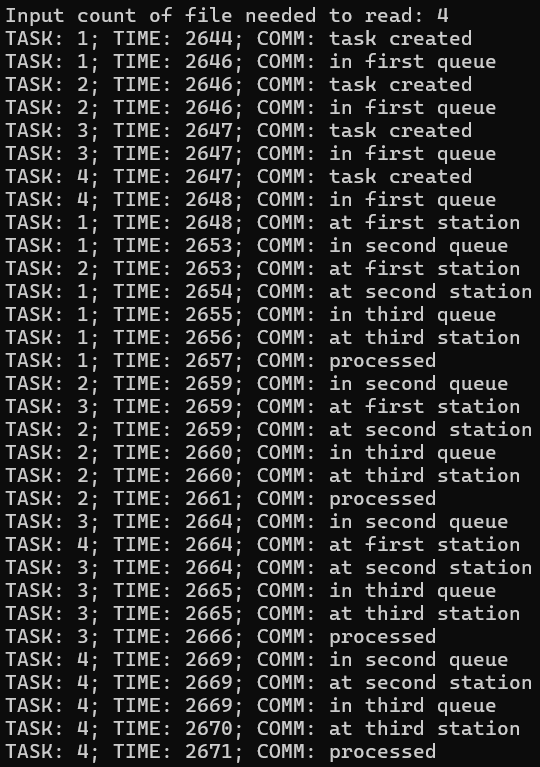
\includegraphics[scale=0.8]{tools/log.png}
	\caption{Лог для четырех задач}
	\label{pic:log}
\end{figure}

Из рисунка \ref{pic:log} видно, что задачи действительно выполняются параллельно. На рисунке \ref{pic:model} представлена
графическая интерпертация работы конвейера:
\clearpage\begin{figure}[h]
	\centering
	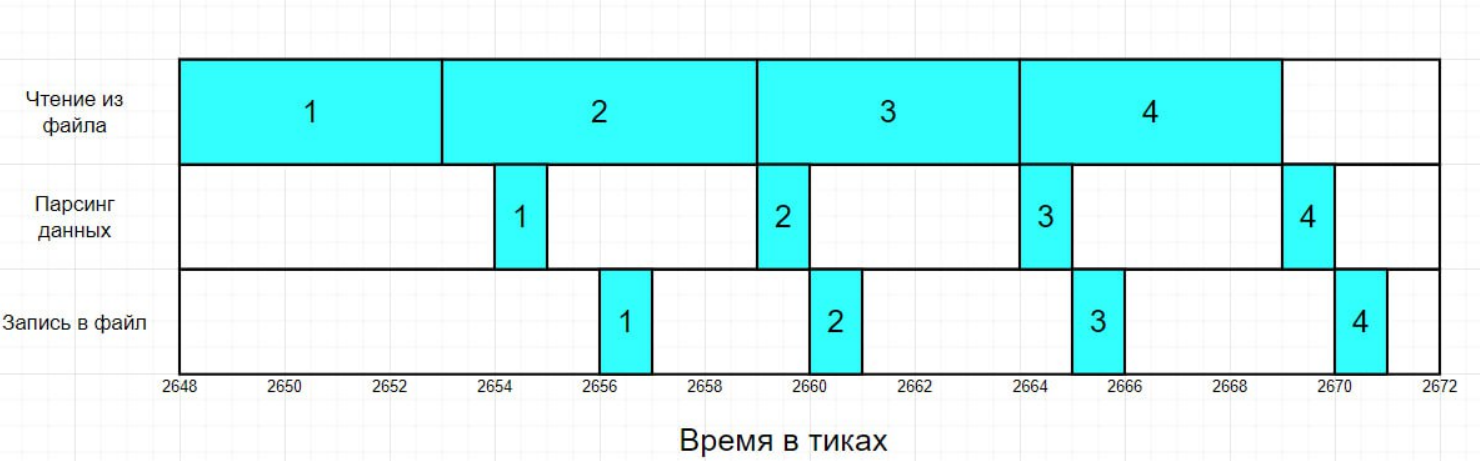
\includegraphics[scale=0.5]{tools/model.png}
	\caption{Графическая интерпретация работы}
	\label{pic:model}
\end{figure}

Можно заметить, что задачи действительно выполняются в параллельном режиме.

На рисунке \ref{pic:stats} представлены некоторые средние статистические показатели:
\begin{figure}[h]
	\centering
	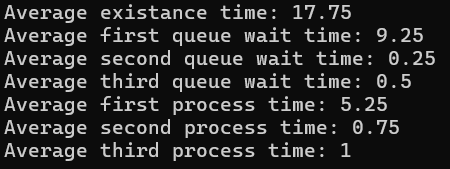
\includegraphics[scale=1.0]{tools/stats.png}
	\caption{Статистические показатели}
	\label{pic:stats}
\end{figure}

Поскольку параметры ожидания в каждой очереди ненулевые, можно сделать вывод, что при конвейерной обработке 
возникают простои.

\clearpage\ssr{ЗАКЛЮЧЕНИЕ}
В ходе выполнения лабораторной работы поставленная цель была достигнута. Были решены все задачи:
\begin{enumerate}
	\item[1)] рассмотрена структура сайта;
	\item[2)] разработан класс, который выполняет парсинг файлов с html кодом и записывает результат в json формате;
	\item[3)] реализован класс-конвейер, который выполняет обработку задач в параллельном режиме;
	\item[4)] проведено исследование, в ходе которого выяснилось, что задачи выполняются параллельно, но иногда
	в процессе обработки возникают простои;
	\item[5)] обоснованы полученные результаты и сделан вывод.
\end{enumerate} 

\addcontentsline{toc}{chapter}{СПИСОК ИСПОЛЬЗОВАННЫХ ИСТОЧНИКОВ}
\renewcommand{\bibname}{СПИСОК ИСПОЛЬЗОВАННЫХ ИСТОЧНИКОВ}
\begin{thebibliography}{}
	\bibitem{parallel}  Энтони Уильямс, C++. Практика многопоточного программирования. --- Город: Санкт-Петербург, 
	Издательский дом «Питер», 2020. --- 640 с.
	\bibitem{threads} Ковалев, Введение в многопоточность / [Электронный ресурс] // Режим доступа: https://rekovalev.site/
	multithreading-3-cpp/\#threads-create
	\bibitem{python3} Язык Python / [Электронный ресурс] // Режим доступа: https://docs.python.org/3/index.html
	\bibitem{pgsql} PostgreSQL / [Электронный ресурс] // Режим доступа: https://www.postgresql.org/
	\bibitem{reciept} Сайт с рецептами / [Электронный ресурс] // Режим доступа: https://www.povareschka.ru/
	\bibitem{time} Функция clock() / [Электронный ресурс] // Режим доступа: https://learn.microsoft.com/ru-ru/\\cpp/c-runtime-library/reference/clock?view=msvc-170
\end{thebibliography}

\end{document}